% Hur är sensorenheten designad?

\section{Sensorenhet}

Sensorenheten har till uppgift att förse huvudenheten med sensordata. Sensordatan den returnerar är obehandlad rådata.

\subsection{Hårdvara}

Sensorenheten består av en Atmega1284p, två reflexsensormoduler och två avståndssensorer. Reflexsensormodulerna är kopplade via två 16-1 muxar till enkretsdatorn. Den ena muxen används för att styra en konstant hög enable-signal till rätt reflexsensor och den andra för att välja rätt utsignal. Båda muxarna styrs av samma styrsignal från enkretsdatorn. Avståndssensorerna är kopplade direkt till enkretsdatorn. Enkretsdatorn är ansluten till huvudenheten med en \todo{20lol-pinnarskabel?} över vilken de kommunicerar via SPI. Figur \ref{sensor-oversikt} illustrerar hur enheten är organiserad i grova drag. \todo{Hänvisa till kopplingsschema i Bilaga}

\begin{figure}[h!]
	\centering
	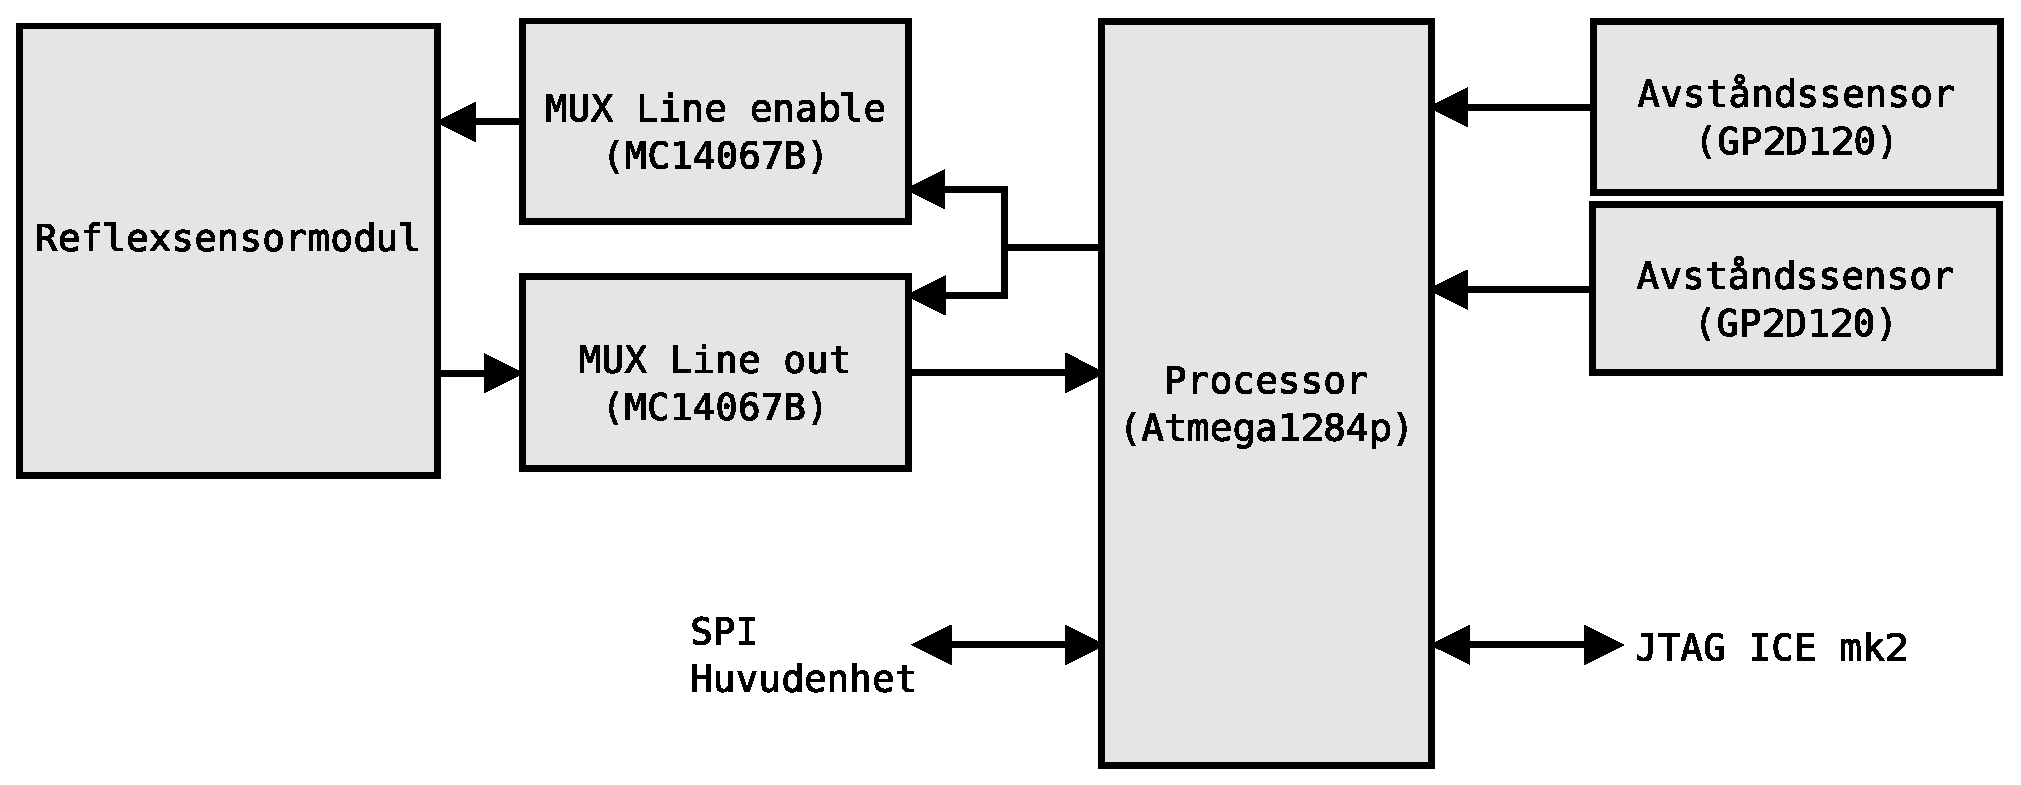
\includegraphics[scale=0.4]{grafik/sensorenhet-oversikt}
	\caption{Översikt av sensorenheten \todo{Lägg till Reflexsensormodul 2}} \label{sensor-oversikt}
\end{figure}

\subsubsection{Reflexsensormodul}
Reflexsensormodulerna består av 11 reflexsensorer var. De ansluts med en 22-pinnars flatkabel vardera där respektive kabel har en enable- och en utsignal för vardera reflexsensor enligt databladet\cite{reflexsensormodul}. De matas med 5V och ger en analog insignal mellan 0V och 5V beroende på hur mycket ljus som reflekteras. De ger låg utspänning då underlaget reflekterar mycket ljus, och hög utspänning då lite ljus reflekteras \todo{Hade vart nice med en graf över lästa värden}.

Den ena reflexsensormodulen används för att detektera vart på banan vi är för att kunna reglera styrningen, endast de två yttersta sensorerna används på den andra modulen för att detektera när en uppplocknings-/nedsättningsstation befinner sig mitt under roboten, de övriga sensorerna används inte.

\subsubsection{Avståndssensorer}
Avståndssensorerna är av typen GP2D120 vilken använder ljus för att detektera avståndet. Dess utsignal är en analog spänning mellan 0V och 3.2V som går hög ju närmare ett objekt befinner sig. \todo{Hade vart nice med en graf}

Avståndssensorerna sitter på vardera sida av roboten och används för att detektera huruvida det står ett paket vid en station eller inte.

\subsection{Processor}
Den centrala komponenten i Sensorenheten är enkretsdatorn Atmega1284p. Den kör en klockfrekvens på 16MHz och utför den faktiska läsningen av sensorerna och vidarebefodrar dessa värden till Huvudenheten. Figur \ref{sensor-processor} visar hur de olika enheterna är kopplade till enkretsdatorn.

\begin{figure}[h!]
	\centering
	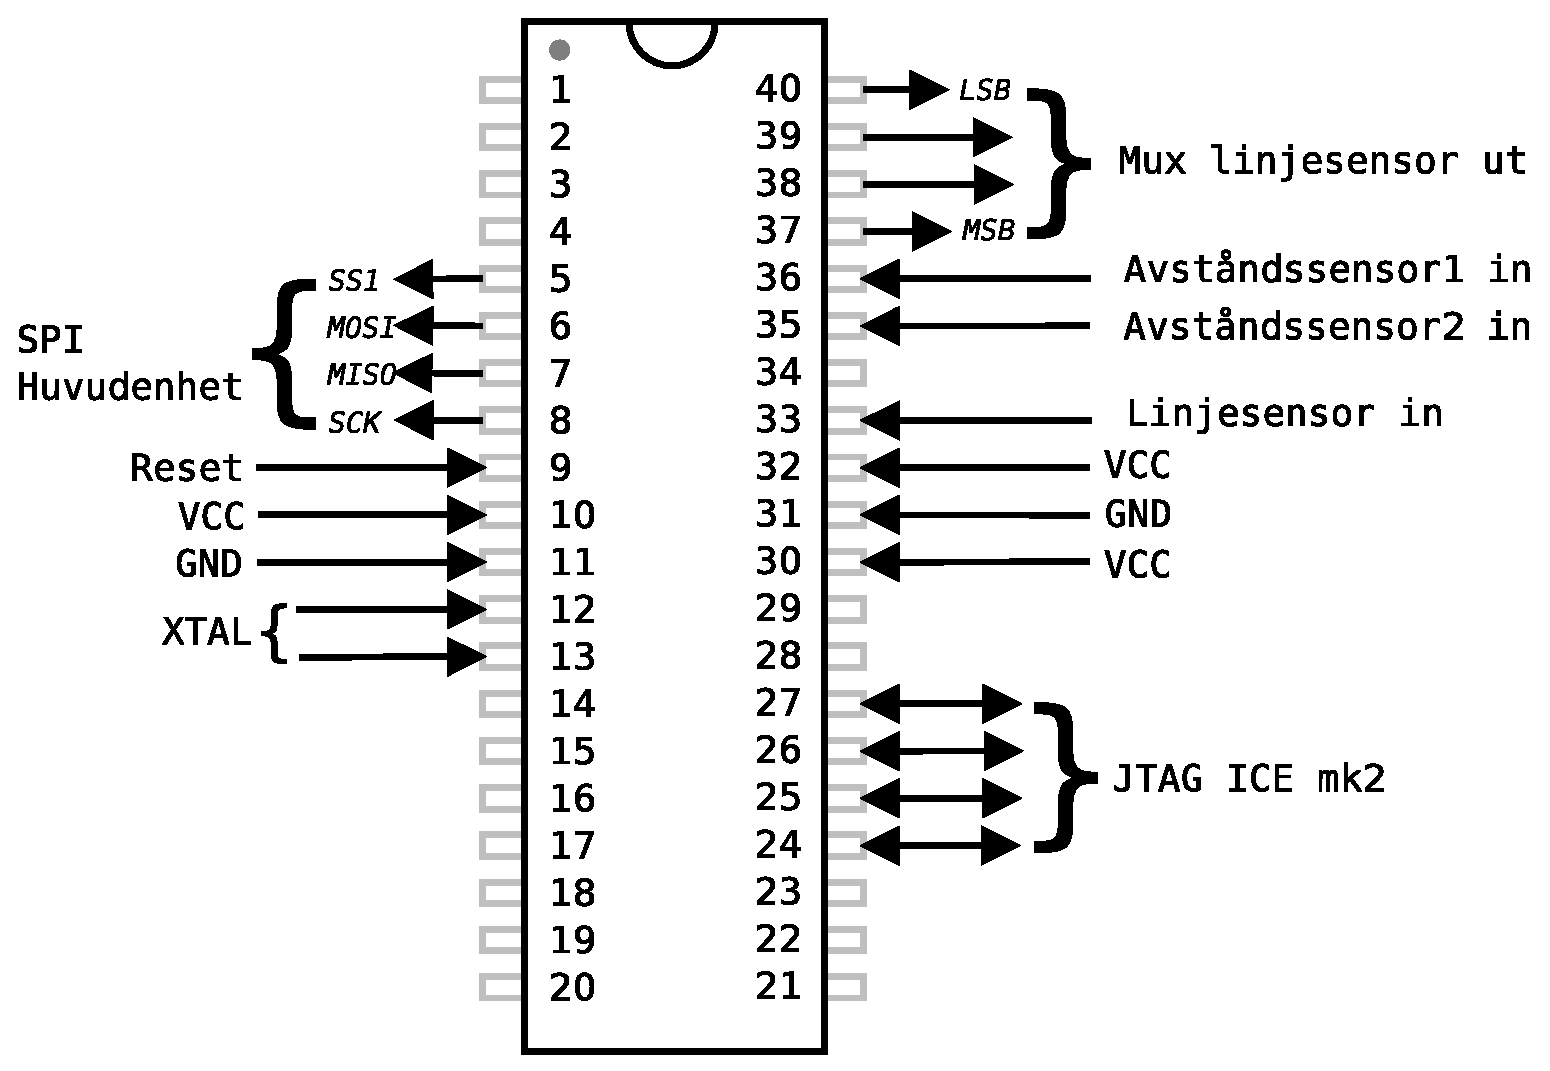
\includegraphics[scale=0.5]{grafik/sensorenhet-processor}
	\caption{Schema över hur enkretssdatorn i sensorenheten är ansluten till övrig hårdvara.} \label{sensor-processor}
\end{figure}

\subsection{Mjukvara}

All mjukvara på sensorenheten är skriven i $C$ och finns på enkretsdatorn. Den består av två delar, illustrerat i figur \ref{sensorenhet-mjukvara}.

\begin{figure}[h!]
	\centering
	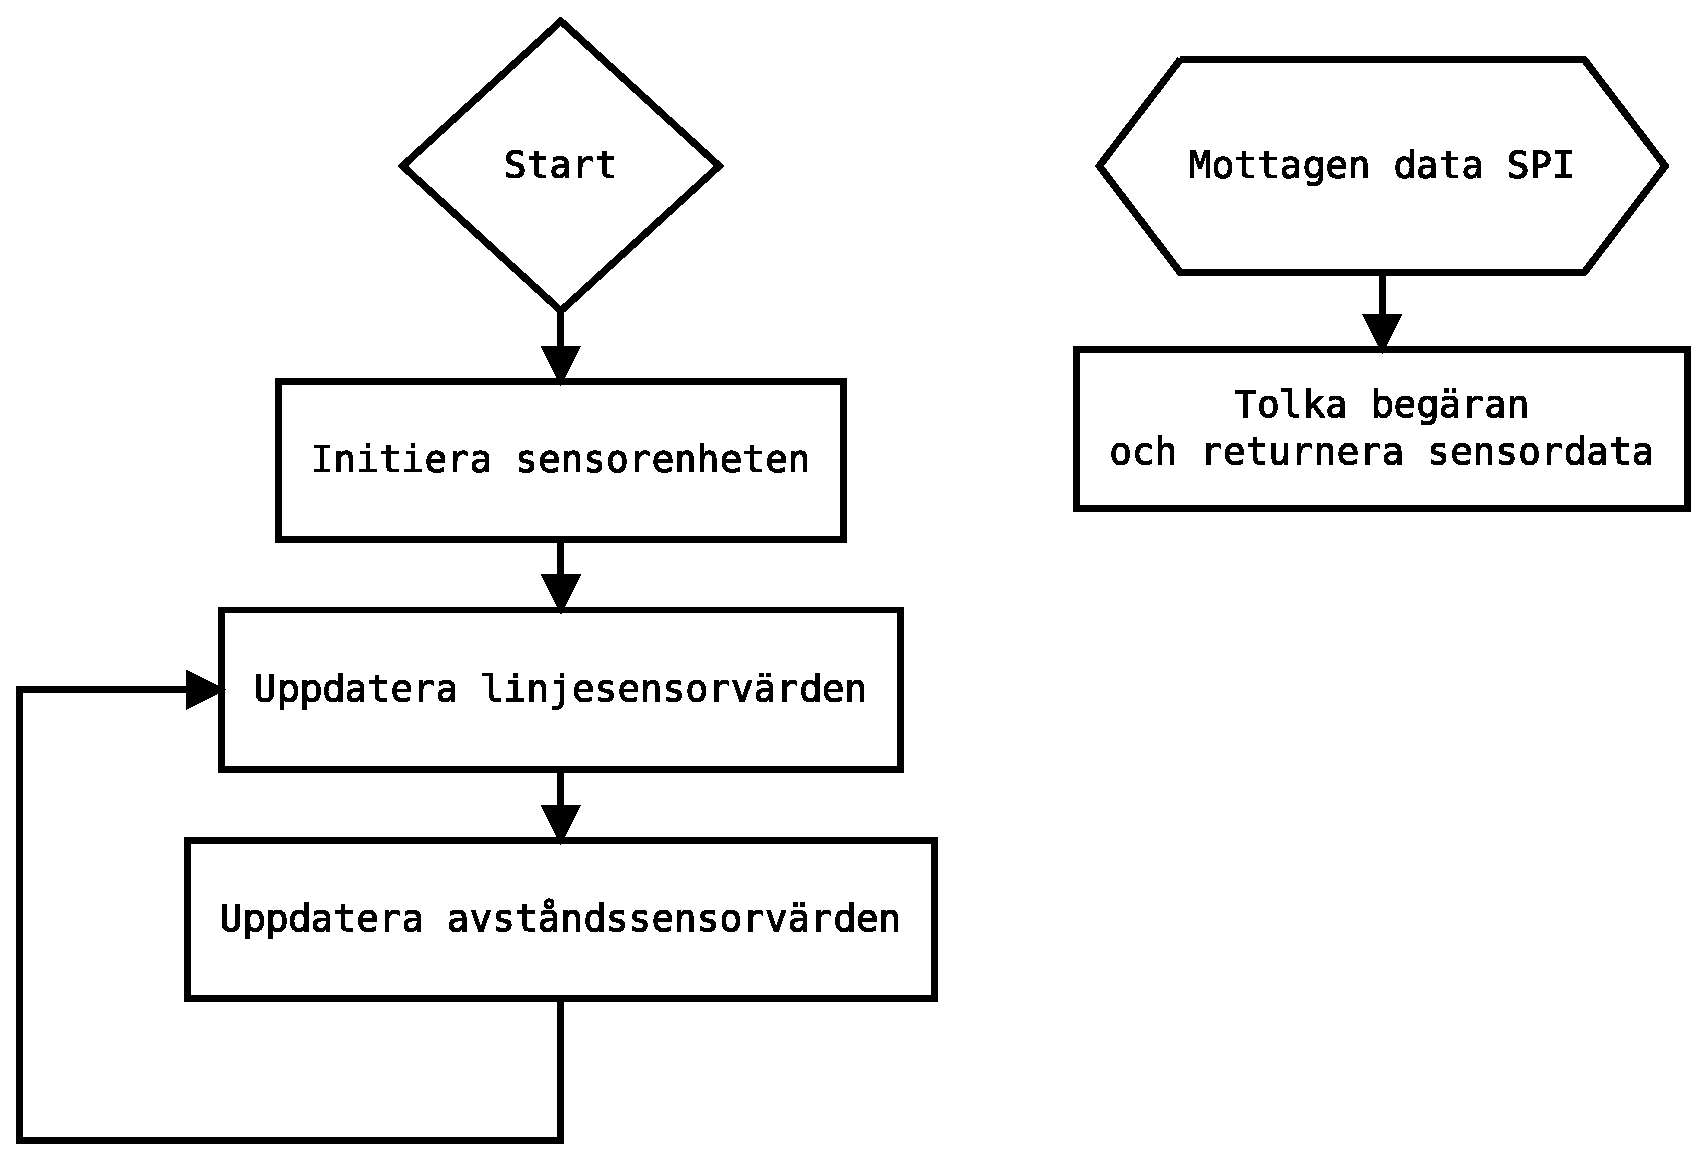
\includegraphics[scale=0.4]{grafik/sensorenhet-mjukvara}
	\caption{Till vänster sensorenhetens \todo{huvudslinga}, till höger den avbrottsrutin som körs vid mottagen data över SPI.} \label{sensorenhet-mjukvara}
\end{figure}

För det första körs en mainloop där sensordata kontinuerligt uppdateras. Först itererar vi igenom Reflexsensorerna genom att först styra om enable-signalen till den aktuella sensorn och därefter utföra en AD-omvandling på den signal vi får tillbaks och sedan gå till nästa. Därefter utför vi i tur och ordning en AD-omvandling på insignalerna från avståndssensorerna. Alla värden sparas i en global datastruktur.
\newline
För det andra tar sensorenheten emot begäran om sensordata från huvudenheten över SPI. När en sådan förfrågan inkommer triggas ett avbrott i vilket sensorenheten svarar med det aktuella sensorvärdet. Då inget i avläsningen av sensorerna är tidskritiskt behöver vi inte oroa oss för när dessa avbrott kommer.
\todo{Atmegan hårdvarustöd för SPI}
